\section*{Introduction}

% \begin{frame}{Intrusion Detection Use Case}

%     \begin{block}{Intrusion Detection System (IDS)}
%         IDSs monitor the behavior of a system to detect malicious activities.
%     \end{block}
%     \hfill
%     \pause
%     \begin{block}{Collaborative IDSs (CIDSs)}
%         CIDSs share information between \alert<3>{distributed parties} (whether they are automated probes, collection points, or legal entities) to improve the characterization of malicious activities, thus facilitating their detection.
%     \end{block}

% \end{frame}



% \begin{frame}{Scaling Intrusion Detection}
\begin{frame}{Federated Learning Primer}

  \begin{columns}
    \begin{column}{0.4\textwidth}
      \textbf{Federated Learning (FL)}
      \small
      \begin{itemize}[<+->]
        \item Distributed ML paradigm (Google, 2017)~\autocite{mcmahan_Communicationefficientlearningdeep_2017}.
        \item Distributed clients  train a common model without sharing training data.
        \item \alert{Privacy-preserving}: high level of abstraction for the shared models, preventing data leakage.
      \end{itemize}
    \end{column}
    
    \begin{column}{0.6\textwidth}
      \begin{figure}
        \centering
        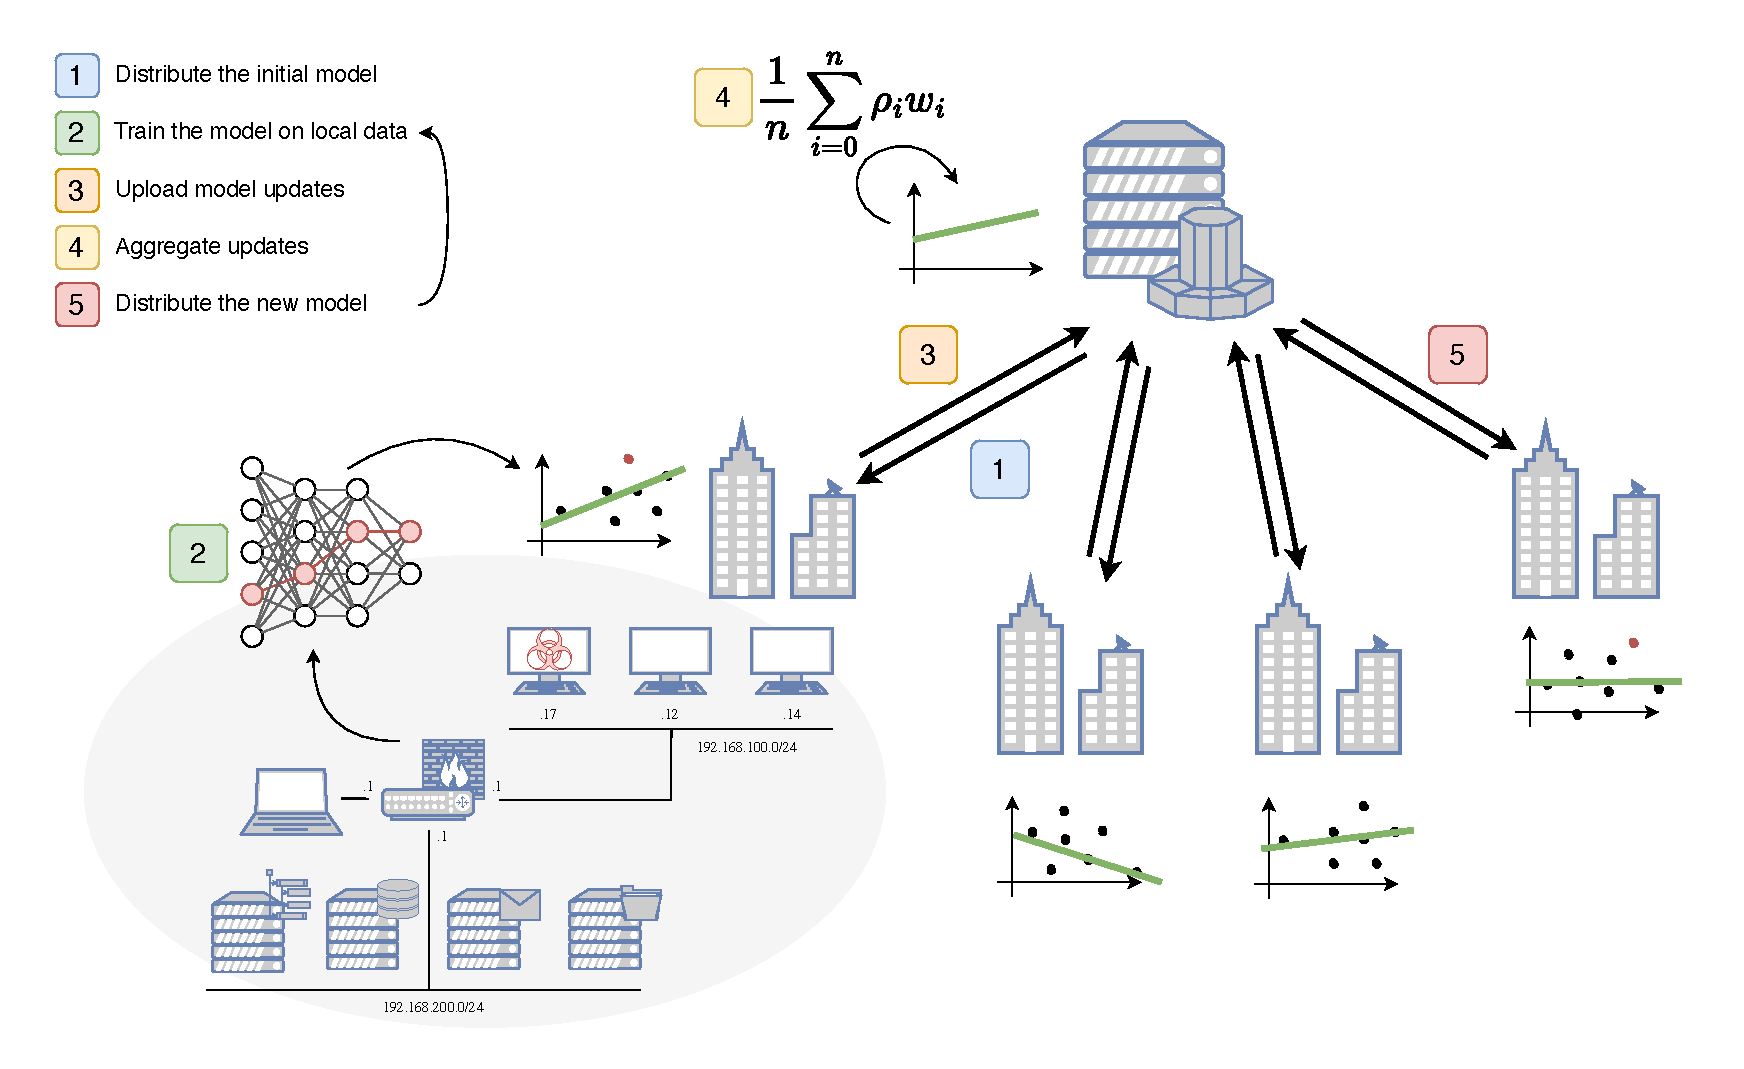
\includegraphics[width=1.1\linewidth,right]{figures/intro/fl.drawio.pdf}
      \end{figure}
    \end{column}
  \end{columns}

  \fcitefootnote{mcmahan_Communicationefficientlearningdeep_2017}
\end{frame}

\begin{frame}{Case Study -- Collaborative IDS}

  \begin{columns}
    \begin{column}{0.4\textwidth}
      \textbf{Collaborative Intrusion Detection between Distributed Organizations}
  \begin{itemize}[<+->]
    \item One NIDS and one monitored network per organization.
    \item \alert{Objective:} improve their local detection performance.
    \item Agree to share knowledge on specific attack classes or devices.
  \end{itemize}
    \end{column}
    
    \begin{column}{0.6\textwidth}
      \begin{figure}
        \centering
        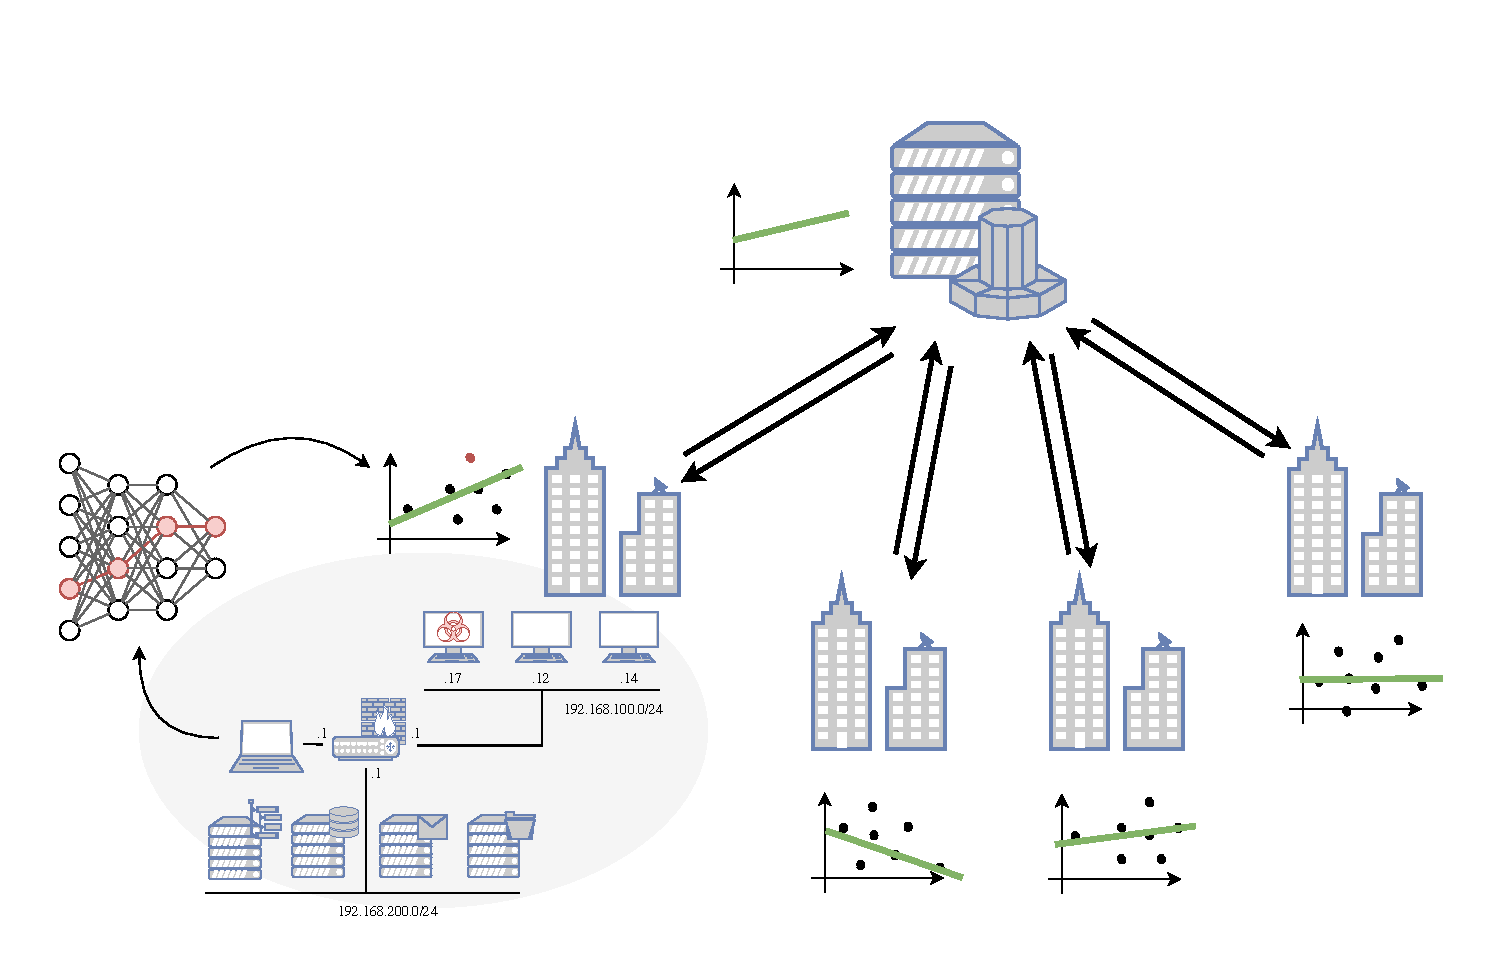
\includegraphics[width=1.1\linewidth,right]{figures/intro/cids.drawio.pdf}
      \end{figure}
    \end{column}
  \end{columns}
\end{frame}



\begin{frame}{Case Study -- Byzantine Contributions}
\begin{columns}
    \begin{column}{0.4\textwidth}
      \begin{itemize}
        \item No guarantees on the quality of the contributions.
        \item Can be intentional, due to poor data quality, or due to data distribution mismatches.
      \end{itemize}
      
      $\rightarrow$ \textbf{Byzantine contributions}
    \end{column}
    
    \begin{column}{0.6\textwidth}
      \begin{figure}
        \centering
        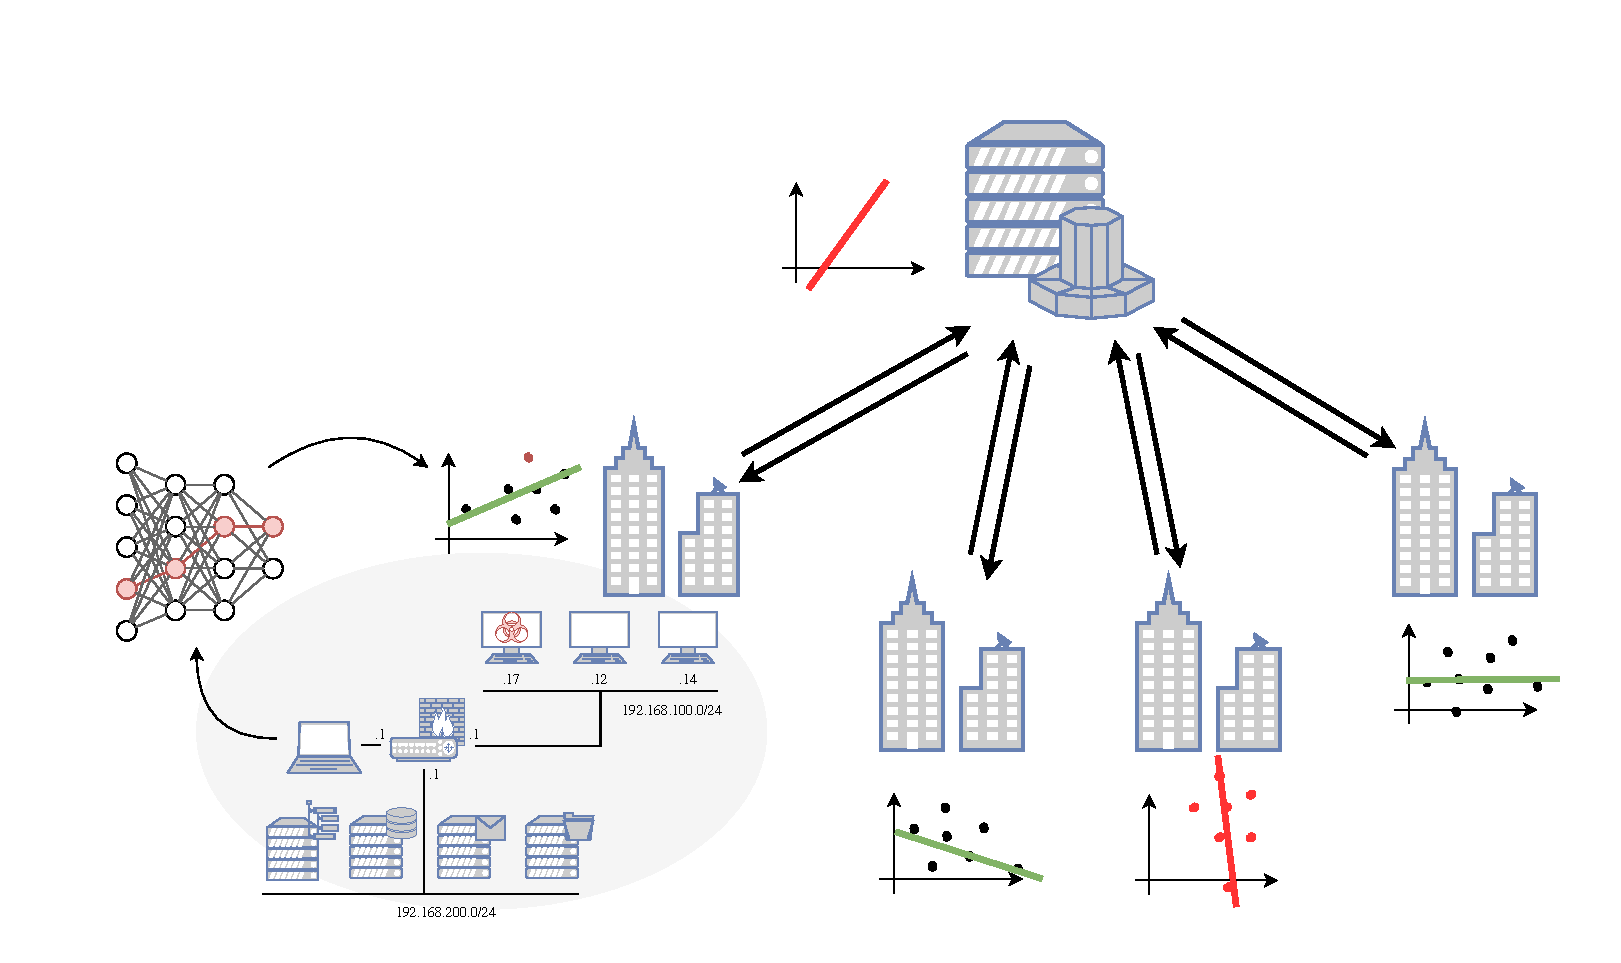
\includegraphics[width=1.1\linewidth,right]{figures/intro/poisoning.drawio.pdf}
      \end{figure}
    \end{column}
  \end{columns}
\end{frame}

\begin{frame}{Case Study -- Generalization}
  \textbf{A cross-silo use case}~\cite{kairouz_AdvancesOpenProblems_2021}:
  \begin{itemize}
    \item few clients (\ie, 10--100);
    \item consequent amount of data, high heterogeneity;
    \item high availability, significant computing resources;
    \item untrusted participants, honest server.
  \end{itemize}
\end{frame}

\begin{frame}{Heterogeneity Headaches}
  
  \begin{columns}
    \begin{column}{.5\textwidth}
      \includegraphics<1>[width=\linewidth]{figures/intro/heterogeneity/introducing_heterogeneity_aggregated.pdf}
      \includegraphics<2>[width=\linewidth]{figures/intro/heterogeneity/introducing_poisoning.pdf}

    \end{column}

    \begin{column}{.5\textwidth}

      \textcolor<2->{lightgray}{%
      \textbf{Challenge I}: \textit{Too much heterogeneity leads to poor performance\dots}
      }
      \only<1>{%
        \begin{itemize} \small
          \item How to handle different feature sets, data distributions?
          \item How to consider models that are dissimilar yet "contain" relevant knowledge?
        \end{itemize}
      }
      \vspace{1ex}


      \textcolor<1>{lightgray}{%
      \textbf{Challenge II}: \textit{Difficult to identify malicious contributions when models are different\dots}
      }
      
      \only<2>{%
        \begin{itemize} \small
          \item Are model "dissimilar" because they are different, or because they are malicious/poisoned?
        \end{itemize}
      }
      \vspace{1ex}
      
    \end{column}
  \end{columns}  
\end{frame}

\begin{frame}{Problem Statement}
% Reformuler 
  \begin{block}{Quality Assessment in Heterogeneous Settings}
    In a context where multiple participants own datasets of \alert{unknown similarity}, each participant contributes a local model update at each round. 
    
    How can one assess the \alert{contribution quality} of each participant’s local models without making assumptions on the \alert{participant data distribution} ?
  \end{block}
  % \begin{block}{Quality Assessment in Heterogeneous Settings}
  %   For $n$ participants $p_i$ and their local datasets $d_i$ of unknown similarity, each participant uploads a model update $w_i^r$ at each round $r$. Given $P = \{ p_1, p_2, \dots, p_n \} $ and $W = \{ w_1^r, w_2^r, \dots, w_n^r \} $, how can one assess the quality of each participant’s contribution without making assumptions on the data distribution across the datasets $d_i$?
  % \end{block}
\end{frame}

\begin{frame}{Existing Solutions}

  \begin{columns}[T]
    
    \begin{column}{.33\textwidth}
      \small\centering
      \textbf{Server-side evaluation}~\autocite{zhou_DifferentiallyPrivateFederated_2022}

      \begin{figure}
        \centering
        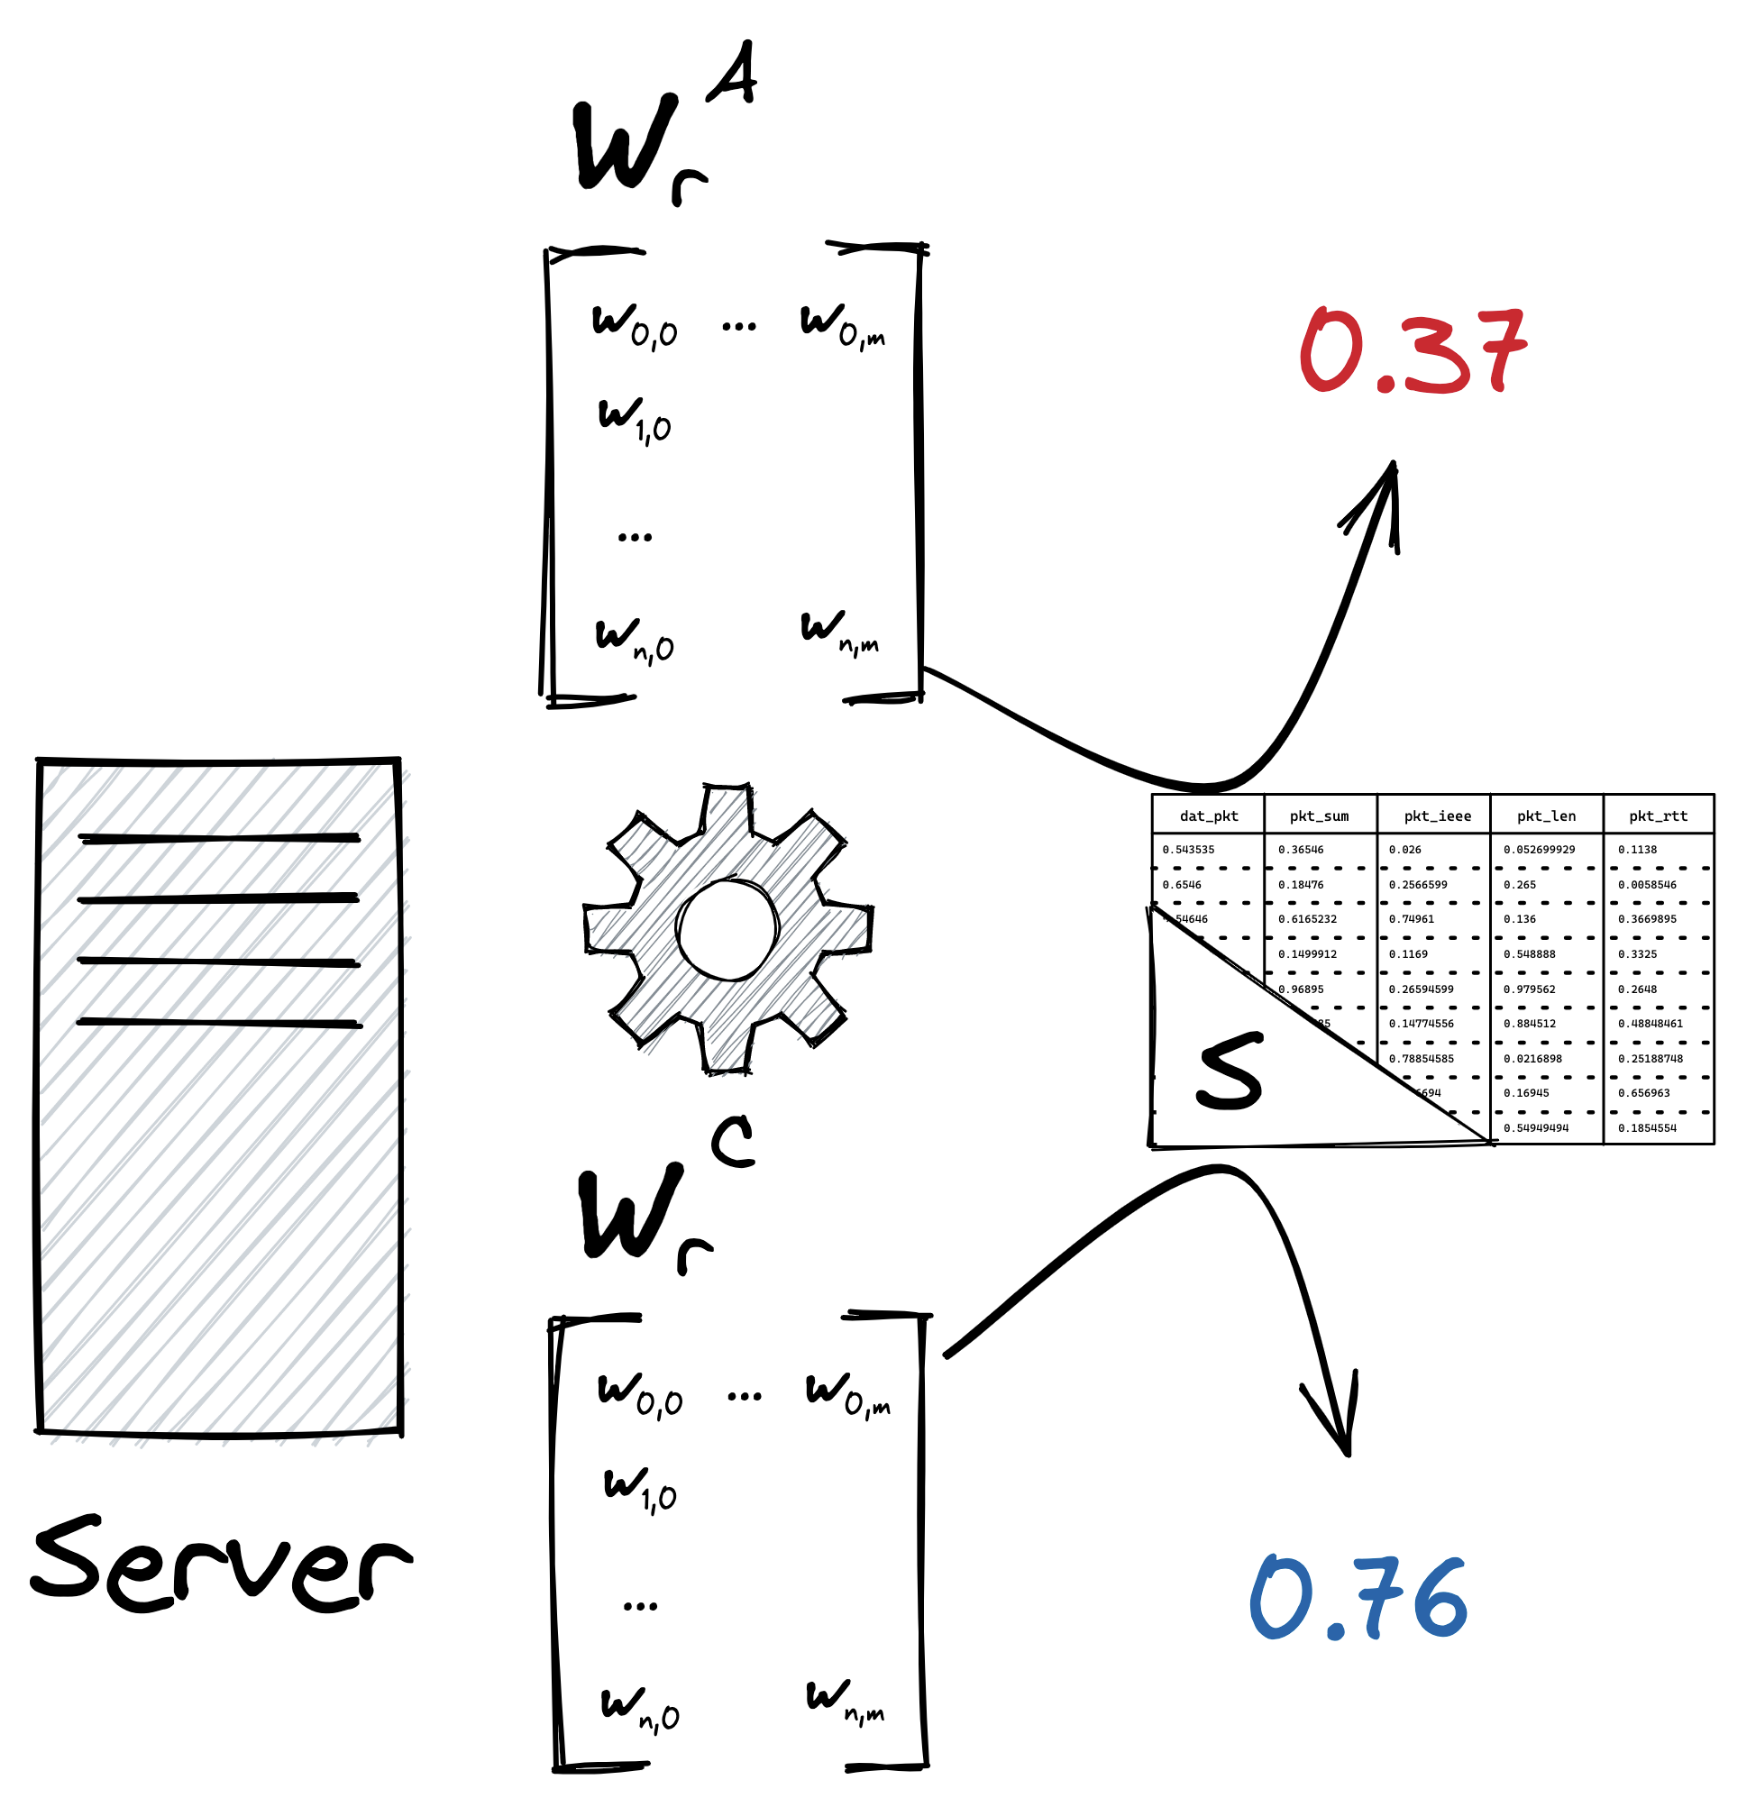
\includegraphics[height=.36\textheight]{figures/radar/server-side-eval}
      \end{figure}

      \begin{itemize}\smaller
        \item Only applicable in IID settings.
        % \item Single source of truth.
      \end{itemize}
    \end{column}

    \onslide<2->{%
      \begin{column}{.33\textwidth}
        \small\centering
        \textbf{Server-side comparison}~\autocite{briggs_Federatedlearninghierarchical_2020}

        \begin{figure}
          \centering
          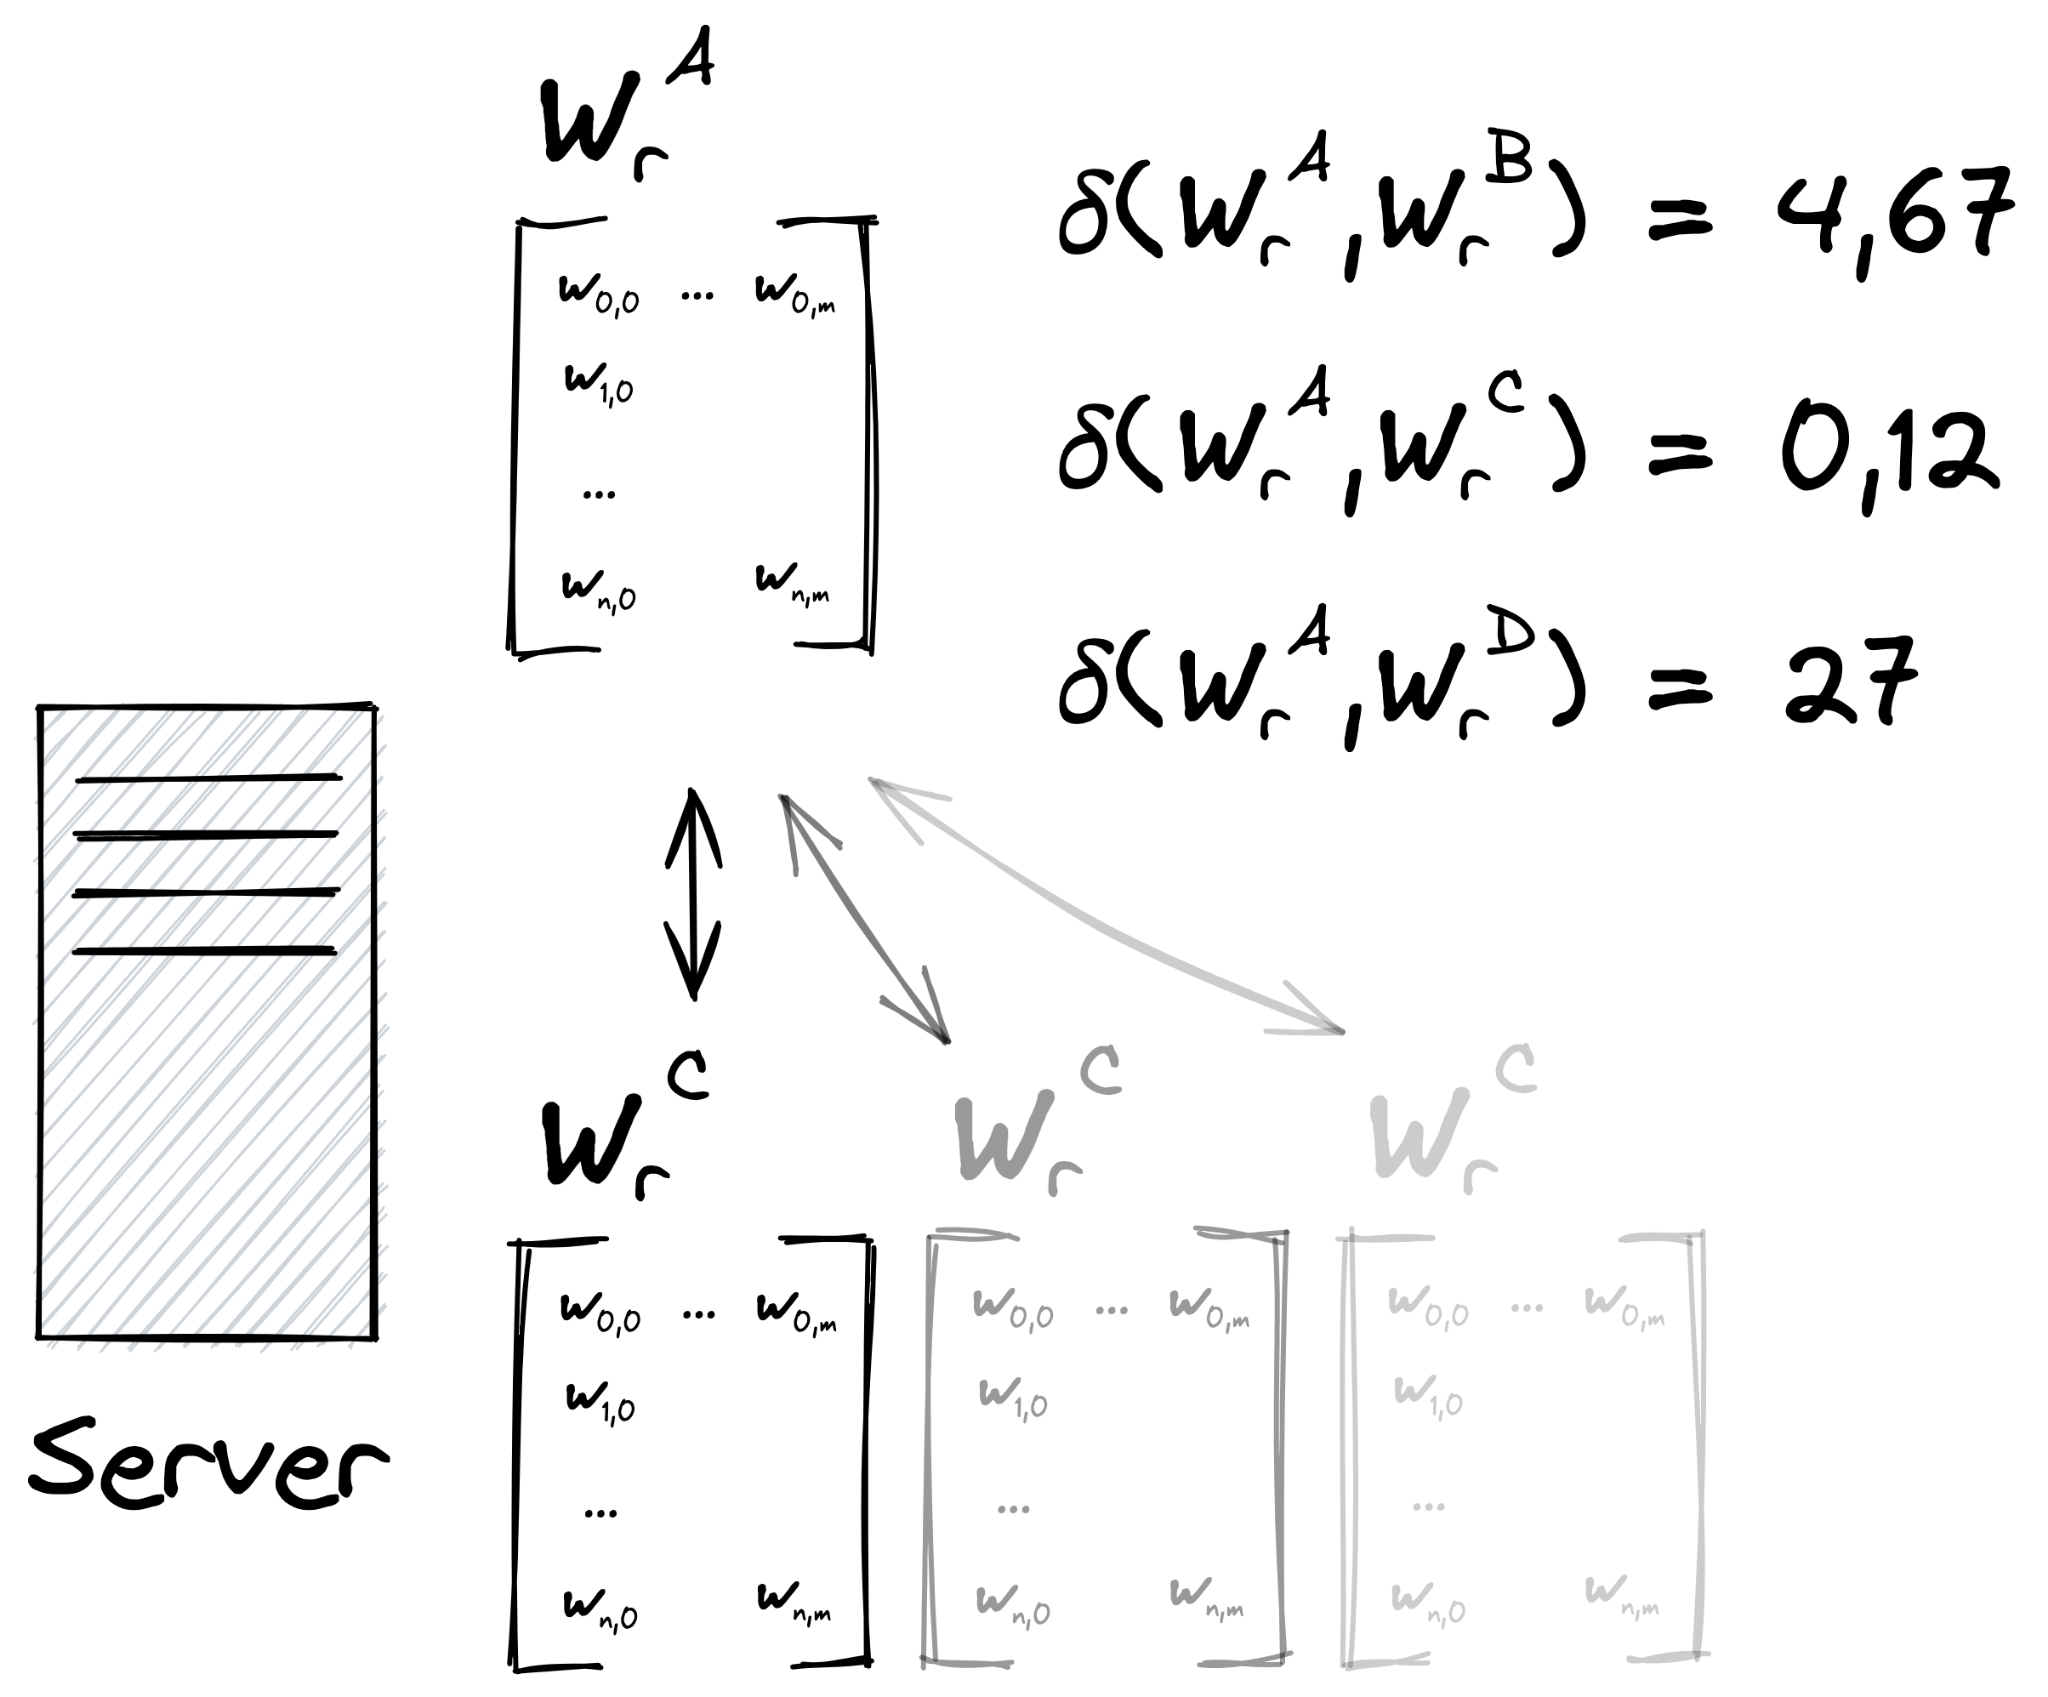
\includegraphics[height=.36\textheight]{figures/radar/server-side-comp}
        \end{figure}

        \begin{itemize}\smaller
          \item Less related to client data.
          % \item More appropriate for high-dimensional data.
        \end{itemize}
      \end{column}%
    }

    \onslide<3->{%
      \begin{column}{.33\textwidth}
        \small\centering
        \textbf{Client-side evaluation}~\autocite{zhao_ShieldingCollaborativeLearning_2020}

        \begin{figure}
          \centering
          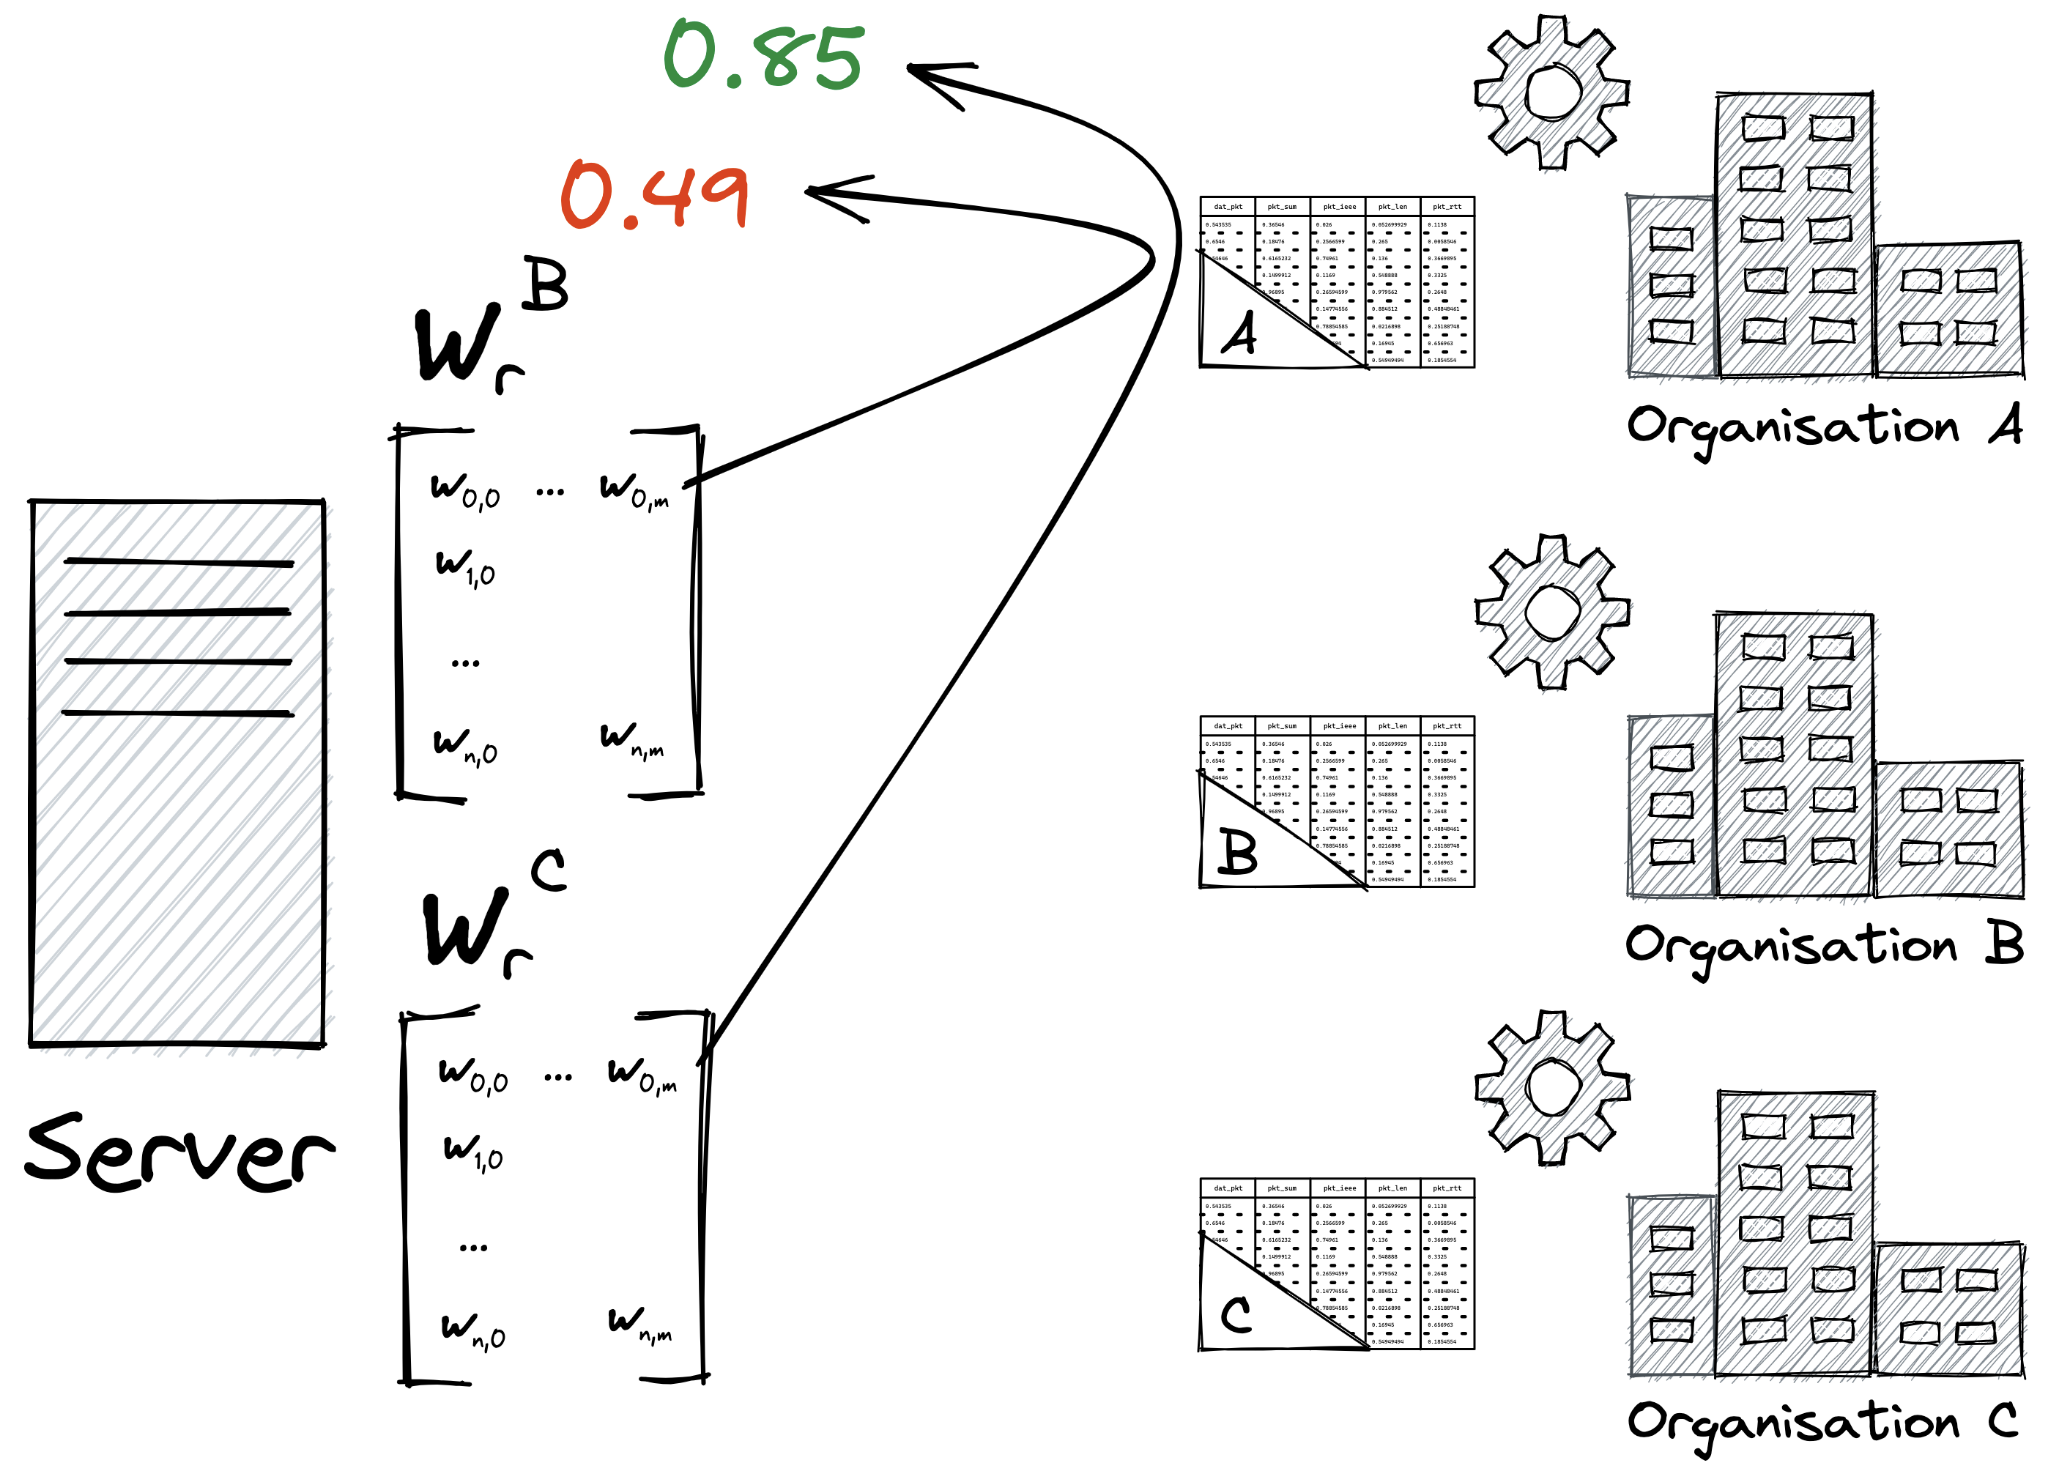
\includegraphics[height=.36\textheight]{figures/radar/client-side-eval}
        \end{figure}

        \begin{itemize}\smaller
          \item High cost in cross-device.
          % \item More susceptible to badmouthing.
        \end{itemize}
      \end{column}%
    }

  \end{columns}

  \vspace{3ex}
  
  \fcitefootnote{zhou_DifferentiallyPrivateFederated_2022}
  \only<1>{\blankfootnote{}} % To keep the same height for the footnotes.
  \only<2->{\fcitefootnote{briggs_Federatedlearninghierarchical_2020}}
  \only<3->{\fcitefootnote{zhao_ShieldingCollaborativeLearning_2020}}

\end{frame}

\begin{frame}{Architecture}
  \centering
    \begin{figure}
        \centering
        \includegraphics<1>[width=.95\linewidth,left]{figures/radar.pdf}%
        \caption*{\texttt{RADAR} architecture. } % remove Figure:
        \label{fig:radar}
    \end{figure}  
         
    % \tableofcontents%[hideallsubsections,]
\end{frame}

